%%%%%%%%% ICML 2021 EXAMPLE LATEX SUBMISSION FILE %%%%%%%%%%%%%%%%%

%\documentclass{article}

%% Optional math commands from https://github.com/goodfeli/dlbook_notation.
%%%%%% NEW MATH DEFINITIONS %%%%%

\usepackage{amsmath,amsfonts,bm}

% Mark sections of captions for referring to divisions of figures
\newcommand{\figleft}{{\em (Left)}}
\newcommand{\figcenter}{{\em (Center)}}
\newcommand{\figright}{{\em (Right)}}
\newcommand{\figtop}{{\em (Top)}}
\newcommand{\figbottom}{{\em (Bottom)}}
\newcommand{\captiona}{{\em (a)}}
\newcommand{\captionb}{{\em (b)}}
\newcommand{\captionc}{{\em (c)}}
\newcommand{\captiond}{{\em (d)}}

% Highlight a newly defined term
\newcommand{\newterm}[1]{{\bf #1}}


% Figure reference, lower-case.
\def\figref#1{figure~\ref{#1}}
% Figure reference, capital. For start of sentence
\def\Figref#1{Figure~\ref{#1}}
\def\twofigref#1#2{figures \ref{#1} and \ref{#2}}
\def\quadfigref#1#2#3#4{figures \ref{#1}, \ref{#2}, \ref{#3} and \ref{#4}}
% Section reference, lower-case.
\def\secref#1{section~\ref{#1}}
% Section reference, capital.
\def\Secref#1{Section~\ref{#1}}
% Reference to two sections.
\def\twosecrefs#1#2{sections \ref{#1} and \ref{#2}}
% Reference to three sections.
\def\secrefs#1#2#3{sections \ref{#1}, \ref{#2} and \ref{#3}}
% Appendix reference, lower-case.
\def\appref#1{appendix~\ref{#1}}
% Appendix reference, capital.
\def\Appref#1{Appendix~\ref{#1}}
% Reference to an equation, lower-case.
\def\eqref#1{equation~\ref{#1}}
% Reference to an equation, upper case
\def\Eqref#1{Equation~\ref{#1}}
% A raw reference to an equation---avoid using if possible
\def\plaineqref#1{\ref{#1}}
% Reference to a chapter, lower-case.
\def\chapref#1{chapter~\ref{#1}}
% Reference to a Chapter, upper case.
\def\Chapref#1{Chapter~\ref{#1}}
\def\twochaprefs#1#2{chapters \ref{#1} and \ref{#2}}
% Reference to a range of chapters
\def\rangechapref#1#2{chapters \ref{#1}--\ref{#2}}
% Reference to a range of chapters, upper case
\def\Rangechapref#1#2{Chapters \ref{#1}--\ref{#2}}
% Reference to an algorithm, lower-case.
\def\algref#1{algorithm~\ref{#1}}
% Reference to an algorithm, upper case.
\def\Algref#1{Algorithm~\ref{#1}}
\def\twoalgref#1#2{algorithms \ref{#1} and \ref{#2}}
\def\Twoalgref#1#2{Algorithms \ref{#1} and \ref{#2}}
% Reference to a part, lower case
\def\partref#1{part~\ref{#1}}
% Reference to a part, upper case
\def\Partref#1{Part~\ref{#1}}
\def\twopartref#1#2{parts \ref{#1} and \ref{#2}}

\def\ceil#1{\lceil #1 \rceil}
\def\floor#1{\lfloor #1 \rfloor}
\def\1{\bm{1}}
\newcommand{\train}{\mathcal{D}}
\newcommand{\valid}{\mathcal{D_{\mathrm{valid}}}}
\newcommand{\test}{\mathcal{D_{\mathrm{test}}}}

\def\eps{{\epsilon}}


% Random variables
\def\reta{{\textnormal{$\eta$}}}
\def\ra{{\textnormal{a}}}
\def\rb{{\textnormal{b}}}
\def\rc{{\textnormal{c}}}
\def\rd{{\textnormal{d}}}
\def\re{{\textnormal{e}}}
\def\rf{{\textnormal{f}}}
\def\rg{{\textnormal{g}}}
\def\rh{{\textnormal{h}}}
\def\ri{{\textnormal{i}}}
\def\rj{{\textnormal{j}}}
\def\rk{{\textnormal{k}}}
\def\rl{{\textnormal{l}}}
% rm is already a command, just don't name any random variables m
\def\rn{{\textnormal{n}}}
\def\ro{{\textnormal{o}}}
\def\rp{{\textnormal{p}}}
\def\rq{{\textnormal{q}}}
\def\rr{{\textnormal{r}}}
\def\rs{{\textnormal{s}}}
\def\rt{{\textnormal{t}}}
\def\ru{{\textnormal{u}}}
\def\rv{{\textnormal{v}}}
\def\rw{{\textnormal{w}}}
\def\rx{{\textnormal{x}}}
\def\ry{{\textnormal{y}}}
\def\rz{{\textnormal{z}}}

% Random vectors
\def\rvepsilon{{\mathbf{\epsilon}}}
\def\rvtheta{{\mathbf{\theta}}}
\def\rva{{\mathbf{a}}}
\def\rvb{{\mathbf{b}}}
\def\rvc{{\mathbf{c}}}
\def\rvd{{\mathbf{d}}}
\def\rve{{\mathbf{e}}}
\def\rvf{{\mathbf{f}}}
\def\rvg{{\mathbf{g}}}
\def\rvh{{\mathbf{h}}}
\def\rvu{{\mathbf{i}}}
\def\rvj{{\mathbf{j}}}
\def\rvk{{\mathbf{k}}}
\def\rvl{{\mathbf{l}}}
\def\rvm{{\mathbf{m}}}
\def\rvn{{\mathbf{n}}}
\def\rvo{{\mathbf{o}}}
\def\rvp{{\mathbf{p}}}
\def\rvq{{\mathbf{q}}}
\def\rvr{{\mathbf{r}}}
\def\rvs{{\mathbf{s}}}
\def\rvt{{\mathbf{t}}}
\def\rvu{{\mathbf{u}}}
\def\rvv{{\mathbf{v}}}
\def\rvw{{\mathbf{w}}}
\def\rvx{{\mathbf{x}}}
\def\rvy{{\mathbf{y}}}
\def\rvz{{\mathbf{z}}}

% Elements of random vectors
\def\erva{{\textnormal{a}}}
\def\ervb{{\textnormal{b}}}
\def\ervc{{\textnormal{c}}}
\def\ervd{{\textnormal{d}}}
\def\erve{{\textnormal{e}}}
\def\ervf{{\textnormal{f}}}
\def\ervg{{\textnormal{g}}}
\def\ervh{{\textnormal{h}}}
\def\ervi{{\textnormal{i}}}
\def\ervj{{\textnormal{j}}}
\def\ervk{{\textnormal{k}}}
\def\ervl{{\textnormal{l}}}
\def\ervm{{\textnormal{m}}}
\def\ervn{{\textnormal{n}}}
\def\ervo{{\textnormal{o}}}
\def\ervp{{\textnormal{p}}}
\def\ervq{{\textnormal{q}}}
\def\ervr{{\textnormal{r}}}
\def\ervs{{\textnormal{s}}}
\def\ervt{{\textnormal{t}}}
\def\ervu{{\textnormal{u}}}
\def\ervv{{\textnormal{v}}}
\def\ervw{{\textnormal{w}}}
\def\ervx{{\textnormal{x}}}
\def\ervy{{\textnormal{y}}}
\def\ervz{{\textnormal{z}}}

% Random matrices
\def\rmA{{\mathbf{A}}}
\def\rmB{{\mathbf{B}}}
\def\rmC{{\mathbf{C}}}
\def\rmD{{\mathbf{D}}}
\def\rmE{{\mathbf{E}}}
\def\rmF{{\mathbf{F}}}
\def\rmG{{\mathbf{G}}}
\def\rmH{{\mathbf{H}}}
\def\rmI{{\mathbf{I}}}
\def\rmJ{{\mathbf{J}}}
\def\rmK{{\mathbf{K}}}
\def\rmL{{\mathbf{L}}}
\def\rmM{{\mathbf{M}}}
\def\rmN{{\mathbf{N}}}
\def\rmO{{\mathbf{O}}}
\def\rmP{{\mathbf{P}}}
\def\rmQ{{\mathbf{Q}}}
\def\rmR{{\mathbf{R}}}
\def\rmS{{\mathbf{S}}}
\def\rmT{{\mathbf{T}}}
\def\rmU{{\mathbf{U}}}
\def\rmV{{\mathbf{V}}}
\def\rmW{{\mathbf{W}}}
\def\rmX{{\mathbf{X}}}
\def\rmY{{\mathbf{Y}}}
\def\rmZ{{\mathbf{Z}}}

% Elements of random matrices
\def\ermA{{\textnormal{A}}}
\def\ermB{{\textnormal{B}}}
\def\ermC{{\textnormal{C}}}
\def\ermD{{\textnormal{D}}}
\def\ermE{{\textnormal{E}}}
\def\ermF{{\textnormal{F}}}
\def\ermG{{\textnormal{G}}}
\def\ermH{{\textnormal{H}}}
\def\ermI{{\textnormal{I}}}
\def\ermJ{{\textnormal{J}}}
\def\ermK{{\textnormal{K}}}
\def\ermL{{\textnormal{L}}}
\def\ermM{{\textnormal{M}}}
\def\ermN{{\textnormal{N}}}
\def\ermO{{\textnormal{O}}}
\def\ermP{{\textnormal{P}}}
\def\ermQ{{\textnormal{Q}}}
\def\ermR{{\textnormal{R}}}
\def\ermS{{\textnormal{S}}}
\def\ermT{{\textnormal{T}}}
\def\ermU{{\textnormal{U}}}
\def\ermV{{\textnormal{V}}}
\def\ermW{{\textnormal{W}}}
\def\ermX{{\textnormal{X}}}
\def\ermY{{\textnormal{Y}}}
\def\ermZ{{\textnormal{Z}}}

% Vectors
\def\vzero{{\bm{0}}}
\def\vone{{\bm{1}}}
\def\vmu{{\bm{\mu}}}
\def\vtheta{{\bm{\theta}}}
\def\va{{\bm{a}}}
\def\vb{{\bm{b}}}
\def\vc{{\bm{c}}}
\def\vd{{\bm{d}}}
\def\ve{{\bm{e}}}
\def\vf{{\bm{f}}}
\def\vg{{\bm{g}}}
\def\vh{{\bm{h}}}
\def\vi{{\bm{i}}}
\def\vj{{\bm{j}}}
\def\vk{{\bm{k}}}
\def\vl{{\bm{l}}}
\def\vm{{\bm{m}}}
\def\vn{{\bm{n}}}
\def\vo{{\bm{o}}}
\def\vp{{\bm{p}}}
\def\vq{{\bm{q}}}
\def\vr{{\bm{r}}}
\def\vs{{\bm{s}}}
\def\vt{{\bm{t}}}
\def\vu{{\bm{u}}}
\def\vv{{\bm{v}}}
\def\vw{{\bm{w}}}
\def\vx{{\bm{x}}}
\def\vy{{\bm{y}}}
\def\vz{{\bm{z}}}

% Elements of vectors
\def\evalpha{{\alpha}}
\def\evbeta{{\beta}}
\def\evepsilon{{\epsilon}}
\def\evlambda{{\lambda}}
\def\evomega{{\omega}}
\def\evmu{{\mu}}
\def\evpsi{{\psi}}
\def\evsigma{{\sigma}}
\def\evtheta{{\theta}}
\def\eva{{a}}
\def\evb{{b}}
\def\evc{{c}}
\def\evd{{d}}
\def\eve{{e}}
\def\evf{{f}}
\def\evg{{g}}
\def\evh{{h}}
\def\evi{{i}}
\def\evj{{j}}
\def\evk{{k}}
\def\evl{{l}}
\def\evm{{m}}
\def\evn{{n}}
\def\evo{{o}}
\def\evp{{p}}
\def\evq{{q}}
\def\evr{{r}}
\def\evs{{s}}
\def\evt{{t}}
\def\evu{{u}}
\def\evv{{v}}
\def\evw{{w}}
\def\evx{{x}}
\def\evy{{y}}
\def\evz{{z}}

% Matrix
\def\mA{{\bm{A}}}
\def\mB{{\bm{B}}}
\def\mC{{\bm{C}}}
\def\mD{{\bm{D}}}
\def\mE{{\bm{E}}}
\def\mF{{\bm{F}}}
\def\mG{{\bm{G}}}
\def\mH{{\bm{H}}}
\def\mI{{\bm{I}}}
\def\mJ{{\bm{J}}}
\def\mK{{\bm{K}}}
\def\mL{{\bm{L}}}
\def\mM{{\bm{M}}}
\def\mN{{\bm{N}}}
\def\mO{{\bm{O}}}
\def\mP{{\bm{P}}}
\def\mQ{{\bm{Q}}}
\def\mR{{\bm{R}}}
\def\mS{{\bm{S}}}
\def\mT{{\bm{T}}}
\def\mU{{\bm{U}}}
\def\mV{{\bm{V}}}
\def\mW{{\bm{W}}}
\def\mX{{\bm{X}}}
\def\mY{{\bm{Y}}}
\def\mZ{{\bm{Z}}}
\def\mBeta{{\bm{\beta}}}
\def\mPhi{{\bm{\Phi}}}
\def\mLambda{{\bm{\Lambda}}}
\def\mSigma{{\bm{\Sigma}}}

% % Tensor
% \DeclareMathAlphabet{\mathsfit}{\encodingdefault}{\sfdefault}{m}{sl}
% \SetMathAlphabet{\mathsfit}{bold}{\encodingdefault}{\sfdefault}{bx}{n}
% \newcommand{\tens}[1]{\bm{\mathsfit{#1}}}
% \def\tA{{\tens{A}}}
% \def\tB{{\tens{B}}}
% \def\tC{{\tens{C}}}
% \def\tD{{\tens{D}}}
% \def\tE{{\tens{E}}}
% \def\tF{{\tens{F}}}
% \def\tG{{\tens{G}}}
% \def\tH{{\tens{H}}}
% \def\tI{{\tens{I}}}
% \def\tJ{{\tens{J}}}
% \def\tK{{\tens{K}}}
% \def\tL{{\tens{L}}}
% \def\tM{{\tens{M}}}
% \def\tN{{\tens{N}}}
% \def\tO{{\tens{O}}}
% \def\tP{{\tens{P}}}
% \def\tQ{{\tens{Q}}}
% \def\tR{{\tens{R}}}
% \def\tS{{\tens{S}}}
% \def\tT{{\tens{T}}}
% \def\tU{{\tens{U}}}
% \def\tV{{\tens{V}}}
% \def\tW{{\tens{W}}}
% \def\tX{{\tens{X}}}
% \def\tY{{\tens{Y}}}
% \def\tZ{{\tens{Z}}}


% Graph
\def\gA{{\mathcal{A}}}
\def\gB{{\mathcal{B}}}
\def\gC{{\mathcal{C}}}
\def\gD{{\mathcal{D}}}
\def\gE{{\mathcal{E}}}
\def\gF{{\mathcal{F}}}
\def\gG{{\mathcal{G}}}
\def\gH{{\mathcal{H}}}
\def\gI{{\mathcal{I}}}
\def\gJ{{\mathcal{J}}}
\def\gK{{\mathcal{K}}}
\def\gL{{\mathcal{L}}}
\def\gM{{\mathcal{M}}}
\def\gN{{\mathcal{N}}}
\def\gO{{\mathcal{O}}}
\def\gP{{\mathcal{P}}}
\def\gQ{{\mathcal{Q}}}
\def\gR{{\mathcal{R}}}
\def\gS{{\mathcal{S}}}
\def\gT{{\mathcal{T}}}
\def\gU{{\mathcal{U}}}
\def\gV{{\mathcal{V}}}
\def\gW{{\mathcal{W}}}
\def\gX{{\mathcal{X}}}
\def\gY{{\mathcal{Y}}}
\def\gZ{{\mathcal{Z}}}

% Sets
\def\sA{{\mathbb{A}}}
\def\sB{{\mathbb{B}}}
\def\sC{{\mathbb{C}}}
\def\sD{{\mathbb{D}}}
% Don't use a set called E, because this would be the same as our symbol
% for expectation.
\def\sF{{\mathbb{F}}}
\def\sG{{\mathbb{G}}}
\def\sH{{\mathbb{H}}}
\def\sI{{\mathbb{I}}}
\def\sJ{{\mathbb{J}}}
\def\sK{{\mathbb{K}}}
\def\sL{{\mathbb{L}}}
\def\sM{{\mathbb{M}}}
\def\sN{{\mathbb{N}}}
\def\sO{{\mathbb{O}}}
\def\sP{{\mathbb{P}}}
\def\sQ{{\mathbb{Q}}}
\def\sR{{\mathbb{R}}}
\def\sS{{\mathbb{S}}}
\def\sT{{\mathbb{T}}}
\def\sU{{\mathbb{U}}}
\def\sV{{\mathbb{V}}}
\def\sW{{\mathbb{W}}}
\def\sX{{\mathbb{X}}}
\def\sY{{\mathbb{Y}}}
\def\sZ{{\mathbb{Z}}}

% Entries of a matrix
\def\emLambda{{\Lambda}}
\def\emA{{A}}
\def\emB{{B}}
\def\emC{{C}}
\def\emD{{D}}
\def\emE{{E}}
\def\emF{{F}}
\def\emG{{G}}
\def\emH{{H}}
\def\emI{{I}}
\def\emJ{{J}}
\def\emK{{K}}
\def\emL{{L}}
\def\emM{{M}}
\def\emN{{N}}
\def\emO{{O}}
\def\emP{{P}}
\def\emQ{{Q}}
\def\emR{{R}}
\def\emS{{S}}
\def\emT{{T}}
\def\emU{{U}}
\def\emV{{V}}
\def\emW{{W}}
\def\emX{{X}}
\def\emY{{Y}}
\def\emZ{{Z}}
\def\emSigma{{\Sigma}}

% entries of a tensor
% Same font as tensor, without \bm wrapper
% \newcommand{\etens}[1]{\mathsfit{#1}}
% \def\etLambda{{\etens{\Lambda}}}
% \def\etA{{\etens{A}}}
% \def\etB{{\etens{B}}}
% \def\etC{{\etens{C}}}
% \def\etD{{\etens{D}}}
% \def\etE{{\etens{E}}}
% \def\etF{{\etens{F}}}
% \def\etG{{\etens{G}}}
% \def\etH{{\etens{H}}}
% \def\etI{{\etens{I}}}
% \def\etJ{{\etens{J}}}
% \def\etK{{\etens{K}}}
% \def\etL{{\etens{L}}}
% \def\etM{{\etens{M}}}
% \def\etN{{\etens{N}}}
% \def\etO{{\etens{O}}}
% \def\etP{{\etens{P}}}
% \def\etQ{{\etens{Q}}}
% \def\etR{{\etens{R}}}
% \def\etS{{\etens{S}}}
% \def\etT{{\etens{T}}}
% \def\etU{{\etens{U}}}
% \def\etV{{\etens{V}}}
% \def\etW{{\etens{W}}}
% \def\etX{{\etens{X}}}
% \def\etY{{\etens{Y}}}
% \def\etZ{{\etens{Z}}}

% The true underlying data generating distribution
\newcommand{\pdata}{p_{\rm{data}}}
% The empirical distribution defined by the training set
\newcommand{\ptrain}{\hat{p}_{\rm{data}}}
\newcommand{\Ptrain}{\hat{P}_{\rm{data}}}
% The model distribution
\newcommand{\pmodel}{p_{\rm{model}}}
\newcommand{\Pmodel}{P_{\rm{model}}}
\newcommand{\ptildemodel}{\tilde{p}_{\rm{model}}}
% Stochastic autoencoder distributions
\newcommand{\pencode}{p_{\rm{encoder}}}
\newcommand{\pdecode}{p_{\rm{decoder}}}
\newcommand{\precons}{p_{\rm{reconstruct}}}

\newcommand{\laplace}{\mathrm{Laplace}} % Laplace distribution

\newcommand{\E}{\mathbb{E}}
\newcommand{\Ls}{\mathcal{L}}
\newcommand{\R}{\mathbb{R}}
\newcommand{\emp}{\tilde{p}}
\newcommand{\lr}{\alpha}
\newcommand{\reg}{\lambda}
\newcommand{\rect}{\mathrm{rectifier}}
\newcommand{\softmax}{\mathrm{softmax}}
\newcommand{\sigmoid}{\sigma}
\newcommand{\softplus}{\zeta}
\newcommand{\KL}{D_{\mathrm{KL}}}
\newcommand{\Var}{\mathrm{Var}}
\newcommand{\standarderror}{\mathrm{SE}}
\newcommand{\Cov}{\mathrm{Cov}}
% Wolfram Mathworld says $L^2$ is for function spaces and $\ell^2$ is for vectors
% But then they seem to use $L^2$ for vectors throughout the site, and so does
% wikipedia.
\newcommand{\normlzero}{L^0}
\newcommand{\normlone}{L^1}
\newcommand{\normltwo}{L^2}
\newcommand{\normlp}{L^p}
\newcommand{\normmax}{L^\infty}

\newcommand{\parents}{Pa} % See usage in notation.tex. Chosen to match Daphne's book.

\DeclareMathOperator*{\argmax}{arg\,max}
\DeclareMathOperator*{\argmin}{arg\,min}

\DeclareMathOperator{\sign}{sign}
\DeclareMathOperator{\Tr}{Tr}
\let\ab\allowbreak


%% Recommended, but optional, packages for figures and better typesetting:
%\usepackage{microtype}
%\usepackage{graphicx}
%\usepackage{wrapfig}
%\usepackage{caption}
%\usepackage{subcaption}
%\usepackage{booktabs} % for professional tables
%\usepackage{amsfonts}       % blackboard math symbols
%\usepackage{amsmath}
%\usepackage{amssymb}
%\usepackage{amsthm}
%\usepackage{nicefrac}       % compact symbols for 1/2, etc.
%\usepackage{xcolor}         %for coloring the text on colorMNIST
%\usepackage{comment}
%\usepackage{enumitem}
%\newtheorem{prop}{Proposition}
%\newcommand{\Xcal}{\mathcal{X}}
%\newcommand{\Bcal}{\mathcal{B}}
%\newcommand{\Ycal}{\mathcal{Y}}
%\newcommand{\Scal}{\mathcal{S}}
%\newcommand{\Lcal}{\mathcal{L}}
%\newcommand{\Dcal}{\mathcal{D}}
%\newcommand{\ie}{i.\,e.}
%\newcommand{\Ie}{I.\,e.}
%\newcommand{\eg}{e.\,g.}
%\newcommand{\Eg}{E.\,g.}
%% \newcommand{\xmark}{\text{\ding{55}}}
%\usepackage{pifont}% http://ctan.org/pkg/pifont
%\newcommand{\cmark}{\ding{51}}%
%\newcommand{\xmark}{\ding{55}}%

%% hyperref makes hyperlinks in the resulting PDF.
%% If your build breaks (sometimes temporarily if a hyperlink spans a page)
%% please comment out the following usepackage line and replace
%% \usepackage{icml2021} with \usepackage[nohyperref]{icml2021} above.
%\usepackage{hyperref}

%% Attempt to make hyperref and algorithmic work together better:
%\newcommand{\theHalgorithm}{\arabic{algorithm}}

%% Use the following line for the initial blind version submitted for review:
%\usepackage{icml2021}

%% If accepted, instead use the following line for the camera-ready submission:
%%\usepackage[accepted]{icml2021}

%% The \icmltitle you define below is probably too long as a header.
%% Therefore, a short form for the running title is supplied here:
%\icmltitlerunning{Appendix}

%\begin{document}

%\twocolumn[
%\icmltitle{APPENDIX:\\
%~\\
%Learning with Perfect Bags:\\
%Addressing Hidden Stratification with Zero Labe led Data}
%\icmlsetsymbol{equal}{*}

%\begin{icmlauthorlist}
%\icmlauthor{Aeiau Zzzz}{to}
%\end{icmlauthorlist}

%\icmlaffiliation{to}{Department of Computation, University of Torontoland, Torontoland, Canada}

%\icmlcorrespondingauthor{Cieua Vvvvv}{c.vvvvv@googol.com}

%\icmlkeywords{semi-supervised learning, dataset bias}

%\vskip 0.3in
%]

%% this must go after the closing bracket ] following \twocolumn[ ...

%\printAffiliationsAndNotice{}  % leave blank if no need to mention equal contribution
%% \printAffiliationsAndNotice{\icmlEqualContribution} % otherwise use the standard text.

%\appendix

% \subsection{Why not use a fair clustering method?}
% Current fair clustering methods \citep{chierichetti2017fair, backurs2019scalable, huang2019coresets} cluster based on the protected attribute and thus are not applicable to our setting in which the deployment set is unlabeled and the training set is incomplete with respect to $s$.

% \begin{figure*}[t]
% \centering
% \includegraphics[width=0.6\textwidth,page=2]{figures/ideal.pdf}
% \caption{Overview of the zero-shot stratification problem. Training dataset (pairs of input data $x$ and class label $y$) will only contain data points that are labeled ``yes'' by the decision policy. This systematic bias might result in a subgroup(s) to have zero labeled data (in the example above, ``married'' subgroup has zero labeled data). The subgrouping information $s$ is unavailable/unlabeled at deployment time, and is only partially labeled at train time.}
% \label{fig:censoring}
% \end{figure*}

\section{Appendix}\label{sec:zsf-appendix}
\subsection{Results for Adult Income}\label{sec:adult-results}
\begin{figure*}[p]
    \centering
    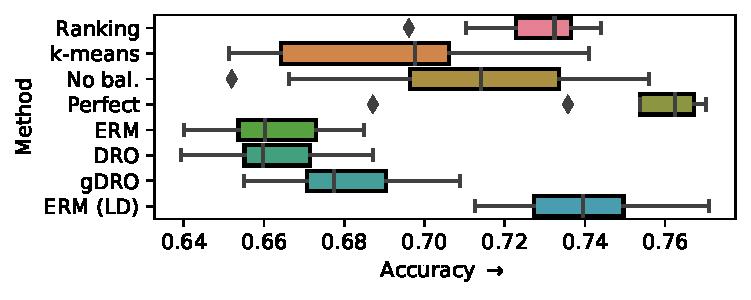
\includegraphics[width=\columnwidth]{figures/adult_partial_acc.pdf}
    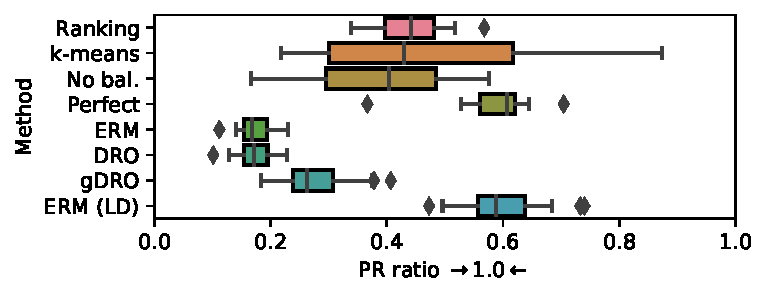
\includegraphics[width=\columnwidth]{figures/adult_partial_prr.pdf}
    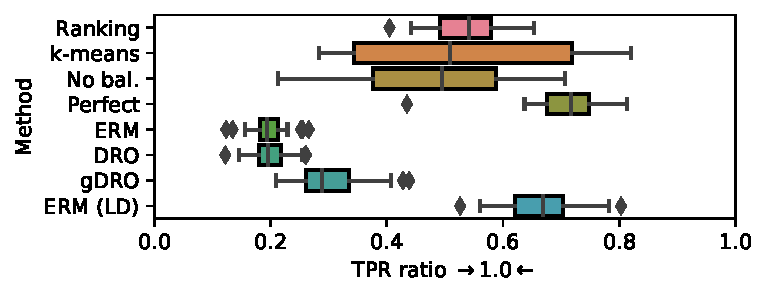
\includegraphics[width=\columnwidth]{figures/adult_partial_tprr.pdf}
    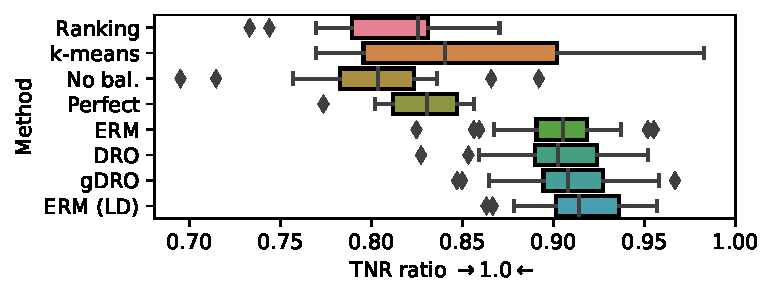
\includegraphics[width=\columnwidth]{figures/adult_partial_tnrr.pdf}
    \caption{%
    Results for the Adult Income dataset with \emph{subgroup bias},
    for the binary classification task of predicting whether an individual earns $>$\$50,000 with a binary subgrouping based on \emph{gender}.
    \texttt{ERM (LD)} refers to a model based on ERM (empirical risk minimization),
    trained on a \textbf{l}abelled \textbf{d}eployment set; thus not suffering from bias in the training set.
    \textbf{Top left}: Accuracy.
    \textbf{Top right}: Positive rate ratio.
    \textbf{Bottom left}: True positive rate ratio.
    \textbf{Bottom right}: True negative rate ratio.
    For the \texttt{Ranking} clustering, the clustering accuracy was 69.7\% $\pm$ 0.3\%;
    for \texttt{K-means} it was 43\% $\pm$ 3\%.
    }%
    \label{fig:adult-subgroup-bias}
\end{figure*}
\begin{figure*}[p]
    \centering
    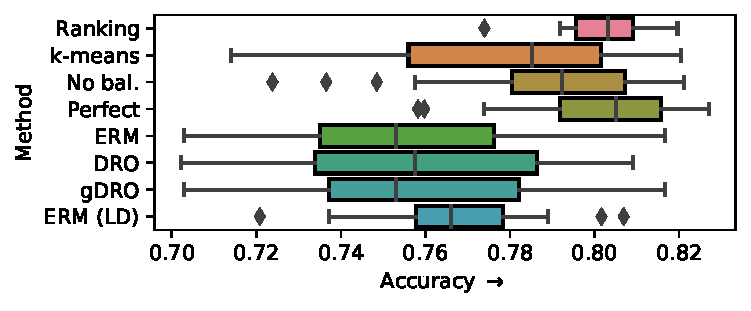
\includegraphics[width=\columnwidth]{figures/adult_miss_s_acc.pdf}
    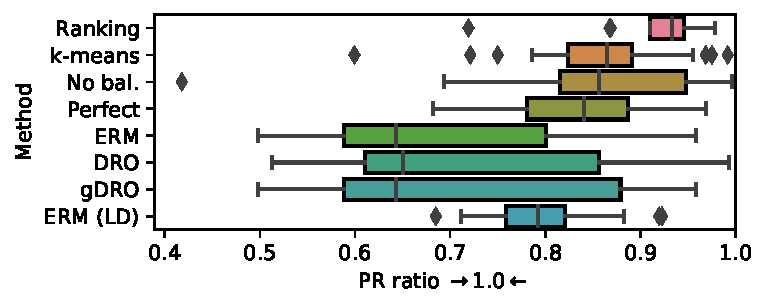
\includegraphics[width=\columnwidth]{figures/adult_miss_s_prr.pdf}
    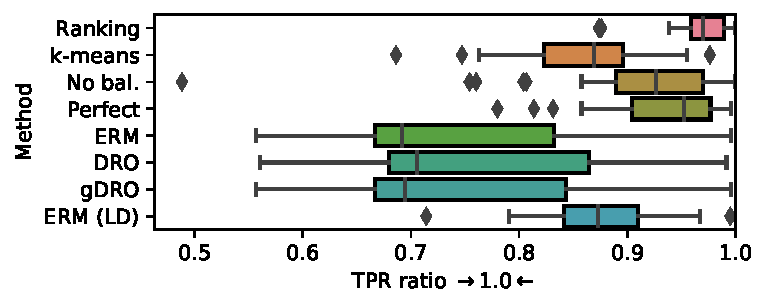
\includegraphics[width=\columnwidth]{figures/adult_miss_s_tprr.pdf}
    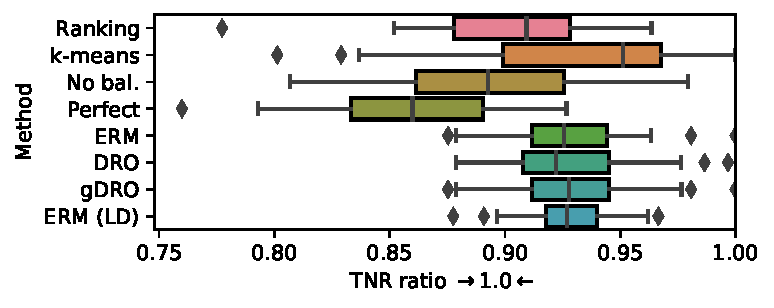
\includegraphics[width=\columnwidth]{figures/adult_miss_s_tnrr.pdf}
    \caption{%
    Results for the Adult Income dataset with a \emph{missing subgroup},
    for the binary classification task of predicting whether an individual earns $>$\$50,000 with a binary subgrouping based on \emph{gender}.
    \texttt{ERM (LD)} refers to a model based on ERM (empirical risk minimization),
    trained on a \textbf{l}abelled \textbf{d}eployment set; thus not suffering from bias in the training set.
    \textbf{Top left}: Accuracy.
    \textbf{Top right}: Positive rate ratio.
    \textbf{Bottom left}: True positive rate ratio.
    \textbf{Bottom right}: True negative rate ratio.
    For the \texttt{Ranking} clustering, the clustering accuracy was 60.4\% $\pm$ 0.8\%;
    for \texttt{K-means} it was 44\% $\pm$ 3\%.
    }%
    \label{fig:adult-missing-subgroup}
\end{figure*}
Figures~\ref{fig:adult-subgroup-bias} and \ref{fig:adult-missing-subgroup} show results from our method on the Adult Income dataset \cite{Dua:2017}.
This dataset is a common dataset for evaluating fair machine learning models. 
Each instance in the dataset is described by $14$ characteristics including gender, education, marital status, number of work hours per week among others, along with a label denoting income level ($\geq$\$50K or not). 
We transform the representation into $62$ real and binary features along with the subgroup label $s$. %%%%%%%%CHECK THESE VALUES%%%%%%%%%%%% 
The dataset is naturally imbalanced with respect to gender: 30\% of the males are labelled as earning more than \$50K per year (high income), while only 11\% of females are labelled as such.
For further details on the dataset construction, see section~\ref{ssec:dataset-construction-adult}.
%
Following standard practice in algorithmic fairness  e.g. \citet{ZemeWuSwePitetal13}, we consider gender to be the subgroup label $s$.

We study the following two settings.
1) \emph{subgroup bias}: we have labelled training data for males ($s=1$) with both positive and negative outcomes, but for the group of females ($s=0$), we only observe the one-sided negative outcome, so the source $\Omega_{y=1,s=0}$ is missing;
2) \emph{missing subgroup}: we have training data for males with positive and negative outcomes, but do not have labelled data for females, i.e.both \ $\Omega_{y=1,s=0}$ and $\Omega_{y=0,s=0}$ are missing.

As before, \texttt{Ranking}, \texttt{k-means}, \texttt{No bal.}\ and \texttt{Perfect} refer to our method with different procedures for constructing (approximately) perfect bags.
As baseline methods, we have \texttt{ERM} (standard empirical risk minimization with balanced batches), \texttt{DRO} \citep{HasSriNamLia18}, \texttt{gDRO} \citep{sagawa2019distributionally}
and \texttt{ERM (LD)} which is the same model as \texttt{ERM}, but trained on the labelled deployment set, in addition to the training set.

In both settings, we observe the same order as for the other dataset in terms of accuracy: \texttt{Perfect} (with ground truth labels for balancing) achieves the highest performance, followed by \texttt{Ranking}, then \texttt{No bal.}, and finally \texttt{k-means}.
However, for the \emph{missing subgroup} setting, \texttt{Ranking} and \texttt{Perfect} are almost identical and the former performs better in terms of de-biasing metrics.
This decreased reliance on balancing can be explained by the additional supervision that comes with having two sources missing instead of one - in order for the discriminator to distinguish between bags from the deployment set and bags from the training set, the former need only contain \emph{one} of the two missing sources.

Generally, we observe a high variance in the results. This is not attributable to our method, however, with the baselines exhibiting the same behaviour, but rather to the fact that the Adult Income dataset is a very noisy dataset which, at the best of times, allows only about 85\% accuracy to be attained (see also \cite{agrawal2020debiasing}). The problem is that samples vary widely in how informative they are. This, coupled with our artificially biasing the dataset to be even more biased (as \emph{subgroup bias} and \emph{missing subgroup}), makes the achievable performance very dependent on which samples the classifier gets to see, which varies according to the random seed used for the data set split.

\subsection{Dataset Construction}\label{sec:dataset-construction}

\subsubsection{Coloured MNIST biasing parameters}
To simulate a real-word setting where the data, labelled or otherwise, is not naturally balanced, we bias the Coloured MNIST training and deployment sets by downsampling certain colour/digit combinations. The proportions of each such combination \emph{retained} in the \emph{subgroup bias} (in which we have one source missing from the training set) and \emph{missing subgroup} (in which we have two sources missing from the training set) are enumerated in table~\ref{color_mnist_biasing_po} and \ref{color_mnist_biasing_id}, respectively.
For the 3-digit-3-colour variant of the problem, no biasing is applied to either the deployment set or the training set (the missing combinations are specified in the caption accompanying figure~\ref{fig:cmnist-3dig-4miss-add}); this variant was experimented with only under the subgroup-bias setting.

\begin{table}[ht]
\caption{Biasing parameters for the training (left) and deployment (right) sets of Coloured MNIST in the \emph{subgroup bias} setting.}
\label{color_mnist_biasing_po}
\centering
\begin{tabular}{lcc}
\toprule
Combination   & \multicolumn{2}{c}{Proportion retained} \\ \cmidrule(lr){2-3}
  & training set & deployment set \\ \midrule
(y = 2, s = {\color{purple}purple}) & 1.0  & 0.7 \\
(y = 2, s = {\color{green}green})   & 0.3  & 0.4 \\
(y = 4, s = {\color{purple}purple}) & 0.0  & 0.2 \\
(y = 4, s = {\color{green}green})   & 1.0  & 1.0 \\
\bottomrule
\end{tabular}
\end{table}

\begin{table}[ht]
\caption{Biasing parameters for the training (left) and deployment (right) sets of Coloured MNIST in the \emph{missing subgroup} setting.}
\label{color_mnist_biasing_id}
\centering
\begin{tabular}{lcc}
\toprule
Combination   & \multicolumn{2}{c}{Proportion retained} \\ \cmidrule(lr){2-3}
  & training set & deployment set \\ \midrule
(y = 2, s = {\color{purple}purple}) & 0.0  & 0.7 \\
(y = 2, s = {\color{green}green})   & 0.85 & 0.6 \\
(y = 4, s = {\color{purple}purple}) & 0.0  & 0.4 \\
(y = 4, s = {\color{green}green})   & 1.0  & 1.0 \\
\bottomrule
\end{tabular}
\end{table}

\subsubsection{Adult Income}\label{ssec:dataset-construction-adult}
For the Adult Income dataset, we do not need to apply any synthetic biasing as the dataset naturally contains some bias wrt $s$. Thus, we instantiate the deployment set as just a random subset of the original dataset. Explicit balancing of the test set is needed to yield meaningful evaluation, however, namely in the penalizing of biased classifiers, but need be taken in doing so. Balancing the test set such that
\begin{align}
    |\{x \in X |s=0, y=0\}| &= |\{x \in X |s=1, y=0\}|    \nonumber\\
    \text{and}~|\{x \in X |s=0, y=1\}| &= |\{x \in X |s=1, y=1\}|
\end{align}
where for both target classes, $y=0$ and $y=1$, the proportions of the groups $s=0$ and $s=1$ are made to be the same, is intuitive, yet at the same time precludes sensible comparison of the accuracy/fairness trade-off of the different classifiers.
Indeed, with the above conditions, a majority classifier (predicting all 1s or 0s) achieves comparable accuracy to the fairness-unaware baselines, while also yielding perfect fairness, by construction.
This observation motivated us to devise an alternative scheme, where we balance the test set according to the following constraints
\begin{align}
    & |\{x \in X |s=0, y=0\}| 
    = |\{x \in X |s=0, y=1\}|  \nonumber \\
    = &|\{x \in X |s=1, y=1\}|
    = |\{x \in X |s=1, y=0\}|~.
 \end{align}
That is, all subsets of $\Scal \times \Ycal$ are made to be equally sized. Under this new scheme the accuracy of the the majority classifier is 50\% for the binary-classification task.


\subsection{Optimization}
\begin{table*}[p]
 \centering
 \caption{Selected hyperparameters for experiments with Coloured MNIST, Adult and CelebA datasets.}
 \label{tab:hparams}
 \begin{tabular}{llll}
 \toprule
 & \textbf{Coloured MNIST} & \textbf{Adult} & \textbf{CelebA}       
 \\ & 2-dig SB / 2-dig MS / 3-dig SB
 \\ \midrule
 Input size  &   $3 \times 32 \times 32$ & $61$ & $3 \times 64 \times 64$ \\  \midrule
 \multicolumn{4}{c}{Autoencoder}                     \\ \midrule
 Levels                      & $4$         & $1$    & $5$\\
 Level depth                 & $2$         & $1$    & $2$\\
 Hidden units / level        & $[32, 64, 128, 256]$ & $[61]$ & $[32, 64, 128, 256, 512]$\\
 Activation                  & GELU        & GELU   & GELU   \\
 Downsampling op.  & Strided Convs. & -- & Strided Convs.\\
 Reconstruction loss         & MSE         & Mixed$^1$  & MSE \\
 Learning rate               & $1 \times 10^{-3}$   & $1 \times 10^{-3}$  & $1 \times 10^{-3}$ \\ \midrule
 \multicolumn{4}{c}{Clustering}                      \\ \midrule
 Batch size                  & $256$      & $1000$  & --\\
 AE pre-training epochs      & $150$        & $100$ & --   \\
 Clustering epochs           & $100$       & $300$  & -- \\
 Self-supervised loss & Cosine + BCE & Cosine + BCE & --\\
 U (for ranking statistics)             & $5$         & $3$     & --    \\   \midrule
 \multicolumn{4}{c}{Distribution Matching}                   \\ \midrule
 Batch size & $1$/$32$/$14$  & $64$   & $32$ \\
 Bag size   & $256$/$8$/$18$ & $32$ & $8$ \\
 Training iterations    & $8\text{k}/8\text{k}/20\text{k}$ & $5\text{k}$ & $15\text{k}$ \\
 Encoding ($z$) size$^2$  & $128$   & $35$  & $128$ \\
 Binarised $z_s$ & \xmark\, / \cmark\, / \cmark & \xmark & \xmark \\
 $y$-predictor weight ($\lambda_1$) & $1$ & $0$ & $1$  \\ 
 $s$-predictor weight ($\lambda_2$) & $1$ & $0$ & $0$  \\ 
 Adversarial weight ($\lambda_3$)   & $1 \times
 10^{-3}$   & $1$   & $1$\\ 
 Stopgradient $\left(\nabla_\theta h_\psi(f_\theta(X^\mathit{dep}))=0\right)$ & \xmark & \cmark & \xmark \\
 \midrule
 \multicolumn{4}{c}{Predictors}   \\ \midrule
 Learning rate  & $3 \times 10^{-4}$ &   $1 \times 10^{-3}$  $ 1 \times 10^{-3}$\\
 \midrule
 \multicolumn{4}{c}{Discriminator}                   \\ \midrule
 Attention mechanism$^3$    & Gated   & Gated & Gated \\
 Hidden units pre-aggregation  & $[256, 256]$  & $[32]$ & $[256, 256]$\\
 Hidden units post-aggregation & $[256, 256]$ & --  & $[256, 256]$ \\
 Embedding dim (for attention) & $32$ & $128$ & $128$ \\
 Activation & GELU & GELU & GELU \\
 Learning rate  & $3 \times 10^{-4}$    & $1 \times 10^{-3}$ & $1 \times 10^{-3}$\\
 Updates / AE update    & $1$  & $3$    & $1$    \\
 \bottomrule
 \multicolumn{4}{l}{\footnotesize $^1$ Cross-entropy is used for categorical features, MSE for continuous features.} \\
  \multicolumn{4}{p{\textwidth}}{\footnotesize $^2$ $|z|$ denotes the combined size of $z_s$ and $z_y$, with the former occupying $\ceil{\text{log}_2(\mathcal{S})}$ dimensions, the latter the remaining } \\
  \multicolumn{4}{p{\textwidth}}{\footnotesize dimensions.} \\
  \multicolumn{4}{p{\textwidth}}{\footnotesize $^3$ The attention mechanism used for computing the sample-weights within a bag. \emph{Gated} refers to gated attention  proposed by
%   \cite{ilse2018attention}, while \emph{SDP} refers to the scaled dot-product attention proposed by \cite{vaswani2017attention}.
  } \\ 
  \multicolumn{4}{p{\textwidth}}{\footnotesize  \cite{ilse2018attention}.} \\ 
 \end{tabular}
\end{table*}

The hyperparameters and architectures for the Autoencoder (\texttt{AE}), Predictor and Discriminator subnetworks used for the experiments with all datasets are detailed in Table \ref{tab:hparams}. All networks are trained using the Adam optimiser \citep{KinBa15}.

For the Coloured MNIST and CelebA datasets, the baseline \texttt{CNN}, \texttt{DRO}, and \texttt{LfF} (in the case of the former) models use an architecture identical to that of the encoder with two exceptions: 1) max-pooling being used for spatial downsampling instead of strided convolutions; 2) the final convolutional layer is followed by a global average pooling layer followed by a fully-connected classification layer. For evaluating our method, we simply train a linear classifier on top of $z_y$; this is sufficient due to linear-separability being enforced during training by the $y$-predictor.
For the Adult Income dataset, we use an MLP made up of a single hidden layer 35 units in size, followed by a SELU activation \citep{klambauer2017self}, as both both the downstream classifier for our method, and as the network architecture of the baselines. 
All baselines and downstream classifiers alike were trained for $60$ epochs with a learning rate of $1 \times 10^{-3}$ and a batch size of $256$.

Since, by design, we do not have labels for all subgroups the model will be tested on, and bias against these missing subgroups is what we aim to avoid, properly validating, and thus conducting hyperparameter selection for models generally, is not straightforward.
We can use estimates of the mutual information between the learned-representation and $s$ and $y$ (which we wish to minimise w.r.t.\ to the former, maximise w.r.t.\ the latter) to guide the process, though optimizing the model w.r.t.\ to these metrics obtained from only the training set does not guarantee generalization to the missing subgroups.
We can, however, additionally measure the entropy of the predictions on the encoded test set and seek to maximise it across all samples, or alternatively train a discriminator of the same kind used for distribution matching as a measure the shift in the latent space between datasets.
We use the latter approach (considering, the learned distance between subspace distributions, accuracy, and reconstruction loss) to inform an extensive grid-search over the hyperparameter space of our model.

For the \texttt{DRO} baseline, we allowed access to the labels of the test set for the purpose of hyperparameters selection, performing a grid-search over multiple splits to avoid overfitting to any particular instantiation.
Specifically, the threshold ($\eta$) parameter for \texttt{DRO} was determined by a grid-search over the space $\{0.01, 0.1, 0.3, 1.0\}$. The same procedure was carried out for selecting the model capacity constant ( $C$) of the related \texttt{gDRO} baseline.

In addition to the losses stated in the distribution matching objective, $\mathcal{L}$, in the main text, we also regularise the encoder by the $\ell^2$ norm of its embedding, multiplied by a small pre-factor, finding this to work better than more complex regularization methods, such as spectral normalization \citep{miyato2018spectral}, for stabilizing training.

\subsection{Visualizations of results}\label{sec:qual-results}
Figures~\ref{fig:attn_maps} and \ref{fig:cmnist-recon} show some additional visualizations for our results.
For details, see the captions.
\begin{figure*}[tb]
  \centering
    \begin{subfigure}[b]{0.49\textwidth}
    
\includegraphics[width=\textwidth]{figures/celeba_attn_map.png}
    \end{subfigure}
    \hfill
    \begin{subfigure}[b]{0.49\textwidth}
    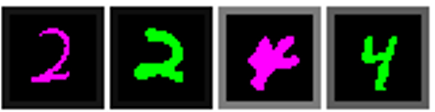
\includegraphics[width=\textwidth]{figures/cmnist_attn_map.png}
    \end{subfigure}
  \caption{
    Example sample-wise attention maps for bags of CelebA (left) and Coloured MNIST (right) images sampled from a balanced deployment set. The training set is biased according to the SB setting where for CelebA ``smiling females'' constitute the missing source and for Colored MNIST {\color{purple}purple} fours constitute the missing source. The attention weights are used during the discriminator's aggregation step to compute a weighted sum over the bag. The attention-weight assigned to each sample is proportional to the lightness of its frame, with black signifying a weight of 0, white a weight of 1. Those samples belonging to the missing subgroup are assigned the highest weight as they signal from which dataset (training vs. deployment) the bag containing them was drawn from.
  }%
  \label{fig:attn_maps}
\end{figure*}

% \subsection{Qualitative results}\label{sec:qual-results}
\begin{figure*}[tb]
  \centering
  \begin{subfigure}[b]{0.39\textwidth}
    \centering
    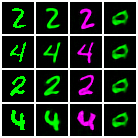
\includegraphics[width=\textwidth]{example_images/fresh-dawn-2179_train_reconstructions_9900.png}
    \caption{
    Different reconstructions on the training set.
    Corresponding to: original, full reconstruction, reconstruction of $z_y$, reconstruction of $z_s$.
    }%
    \label{fig:cmnist-recon-training}
  \end{subfigure}
  % \hfill
  \quad
  \begin{subfigure}[b]{0.39\textwidth}
    \centering
    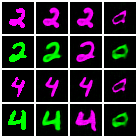
\includegraphics[width=\textwidth]{example_images/fresh-dawn-2179_context_reconstructions_9900.png}
    \caption{
    Different reconstructions on the deployment set.
    Corresponding to: original, full reconstruction, reconstruction of $z_y$, reconstruction of $z_s$.
    }%
    \label{fig:cmnist-recon-deployment}
  \end{subfigure}
  \caption{
   Visualization of our method's solutions for the Coloured MNIST dataset, with {\color{purple}purple} as the missing subgroup.
   In each of the subfigures \ref{fig:cmnist-recon-training} and \ref{fig:cmnist-recon-deployment}:
   Column 1 shows the original images from $x$ from the respective set.
   Column 2 shows plain reconstructions generated from $x_\textit{recon}=g(f_y(x), f_s(x))$.
   Column 3 shows reconstruction with zeroed-out $z_s$: $g(f_y(x), 0)$, which effectively visualises $z_y$.
   Column 4 shows the result of an analogous process where $z_y$ was zeroed out instead.
  }%
  \label{fig:cmnist-recon}
\end{figure*}
% Given a learned invariant representation, we can generate a reconstruction to visualise the information contained in it.
% An example of this can be seen in \figref{fig:3dig-examples}.
% This is from our experiment with 3 digits in Colored MNIST.
% We can clearly see that the reconstructed invariant representation has lost all color information;
% instead all digits are magenta-colored, which was the majority color in the training set.

\subsection{Code}
A \texttt{.zip} file is included containing all files needed to reproduce our experiments. Instructions on how to run them can be found in the \texttt{README.md}.

\subsection{Additional metrics}
Figures~\ref{fig:cmnist-2v4-partial-add}, \ref{fig:cmnist-2v4-miss-s-add},  and \ref{fig:celeba-gender-smiling-add} show the true positive rate (TPR) ratio and the true negative rate (TNR) ratio as additional metrics for Coloured MNIST (2 digits) and CelebA.
These are computed as the ratio of TPR (or TNR) on subgroup $s=0$ over the TPR (or TNR) on subgroup $s=1$; if this gives a number greater than 1, the inverse is taken.
Similarly to the PR ratio reported in the main paper, these ratios give an indication of how much the prediction of the classifier depends on the subgroup label $s$.

Figure~\ref{fig:cmnist-3dig-4miss-add} shows metrics specific to multi-valued $s$ (\ie, non-binary $s$).
We report the minimum (i.e. farthest away from 1) of the pairwise ratios (PR/TPR/TNR ratio min) as well as the largest difference between the raw values (PR/TPR/TNR diff max) . 
Additionally, we compute the Hirschfeld-Gebelein-R\'enyi (HGR) maximal correlation \citep{renyi1959measures} between $S$ and $Y$, serving as a measure of dependence defined between two variables with arbitrary support.
\begin{figure*}[htp]
  \centering
%   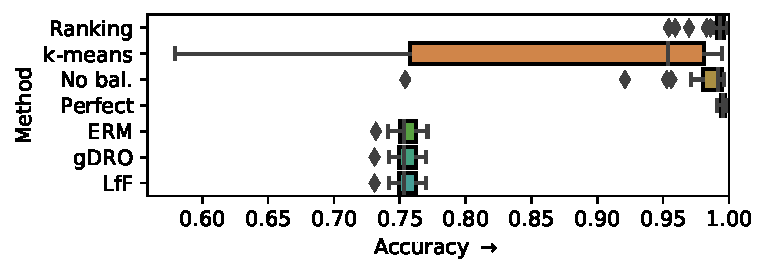
\includegraphics[width=\columnwidth]{figures/cmnist_2v4_partial_acc.pdf}
%   \includegraphics[width=\columnwidth]{figures/cmnist_2v4_partial_pr.pdf}
%   \includegraphics[width=\columnwidth]{figures/cmnist_2v4_partial_tpr.pdf}
%   \includegraphics[width=\columnwidth]{figures/cmnist_2v4_partial_tnr.pdf}
  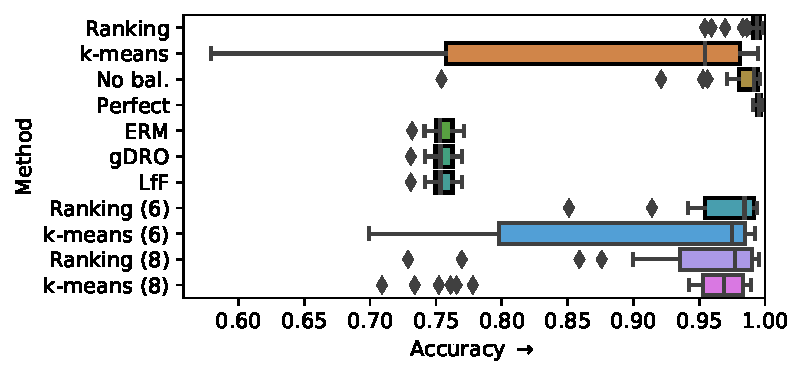
\includegraphics[width=\columnwidth]{figures/cmnist_2v4_partial_overcluster_acc.pdf}
  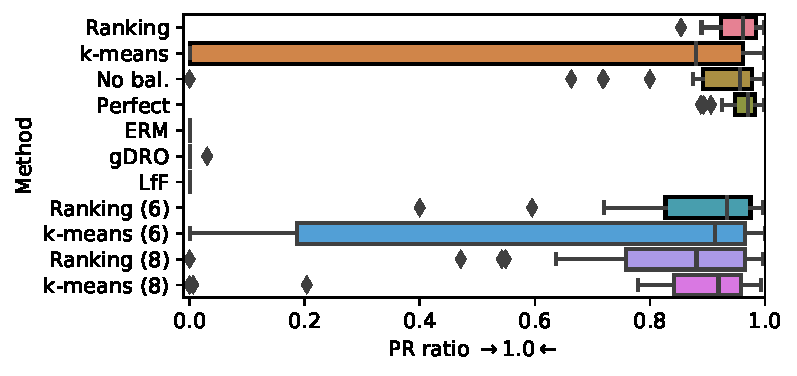
\includegraphics[width=\columnwidth]{figures/cmnist_2v4_partial_overcluster_prr.pdf}
  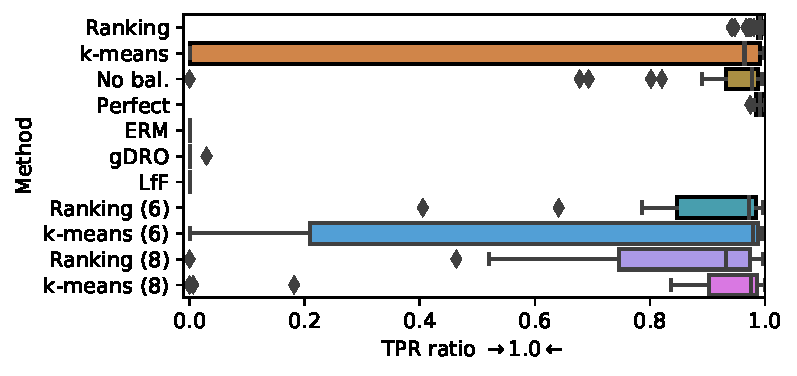
\includegraphics[width=\columnwidth]{figures/cmnist_2v4_partial_overcluster_tprr.pdf}
  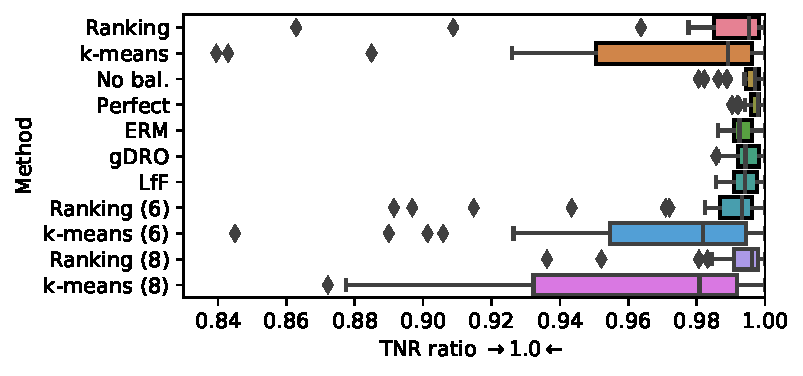
\includegraphics[width=\columnwidth]{figures/cmnist_2v4_partial_overcluster_tnrr.pdf}
  \caption{
    Results from \textbf{30 repeats} for the Coloured MNIST dataset with two digits, 2 and 4, with \emph{subgroup bias} for the colour `{\color{purple}purple}': for {\color{purple}purple}, only the digit class `2' is present.
    \textbf{Top left}: Accuracy.
    \textbf{Top right}: Positive rate ratio.
    \textbf{Bottom left}: True positive rate ratio.
    \textbf{Bottom right}: True negative rate ratio.
    For the \texttt{Ranking} clustering, the clustering accuracy was 96\% $\pm$ 6\%;
    for \texttt{K-means} it was 64\% $\pm$ 10\%.
    For an explanation of \texttt{Ranking (8)} and \texttt{K-means (8)} see section~\ref{sec:overclustering}.
  }%
  \label{fig:cmnist-2v4-partial-add}
\end{figure*}
\begin{figure*}[htp]
  \centering
%   \includegraphics[width=\columnwidth]{figures/cmnist_2v4_miss_s_alt_acc.pdf}
%   \includegraphics[width=\columnwidth]{figures/cmnist_2v4_miss_s_alt_pr.pdf}
%   \includegraphics[width=\columnwidth]{figures/cmnist_2v4_miss_s_alt_tpr.pdf}
%   \includegraphics[width=\columnwidth]{figures/cmnist_2v4_miss_s_alt_tnr.pdf}
  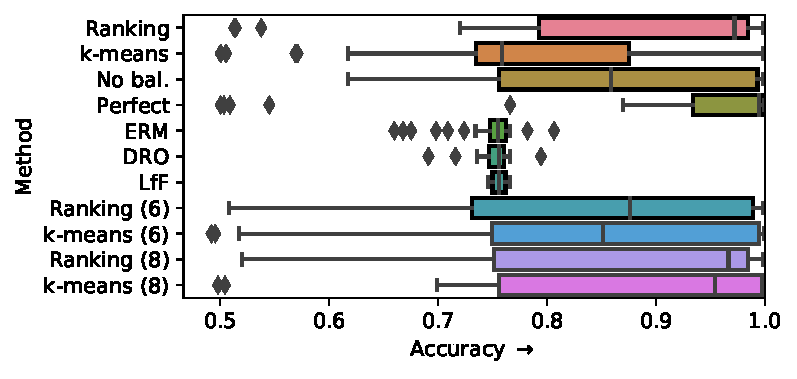
\includegraphics[width=\columnwidth]{figures/cmnist_2v4_miss_s_overcluster_acc.pdf}
  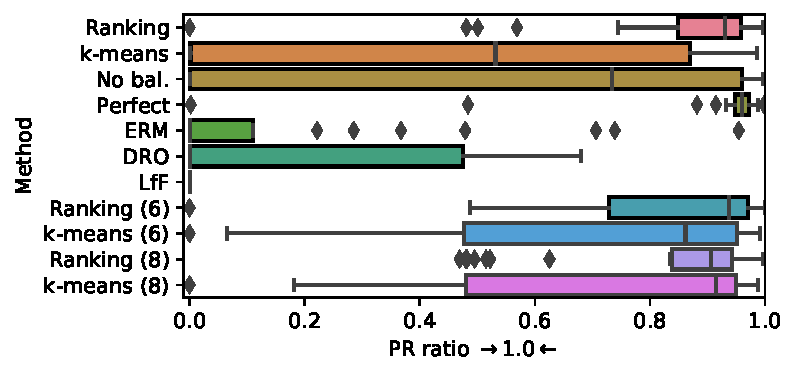
\includegraphics[width=\columnwidth]{figures/cmnist_2v4_miss_s_overcluster_prr.pdf}
  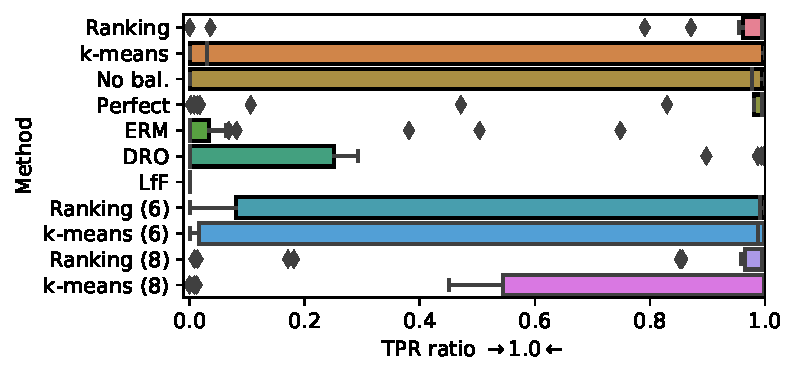
\includegraphics[width=\columnwidth]{figures/cmnist_2v4_miss_s_overcluster_tprr.pdf}
  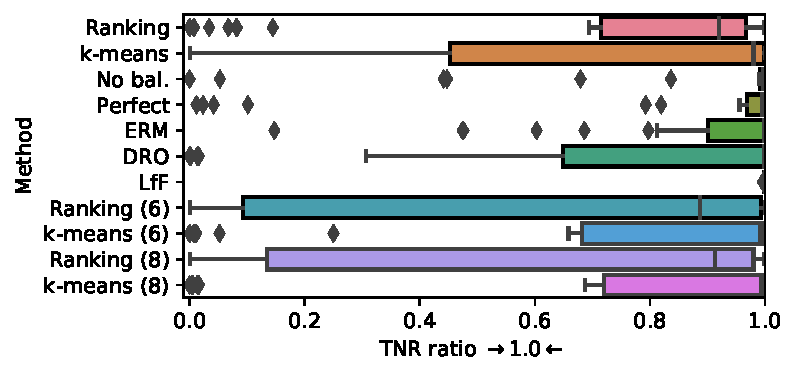
\includegraphics[width=\columnwidth]{figures/cmnist_2v4_miss_s_overcluster_tnrr.pdf}
  \caption{
    Results from \textbf{30 repeats} for the Coloured MNIST dataset with two digits, 2 and 4, with a \emph{missing subgroup}: the training dataset only has {\color{green}green} digits.
    \textbf{Top left}: Accuracy.
    \textbf{Top right}: Positive rate ratio.
    \textbf{Bottom left}: True positive rate ratio.
    \textbf{Bottom right}: True negative rate ratio.
    For the \texttt{Ranking} clustering, the clustering accuracy was 88\% $\pm$ 5\%;
    for \texttt{K-means} it was 72\% $\pm$ 16\%.
    For an explanation of \texttt{Ranking (8)} and \texttt{K-means (8)} see section~\ref{sec:overclustering}.
  }%
  \label{fig:cmnist-2v4-miss-s-add}
\end{figure*}
\begin{figure*}[htp]
  \centering
%   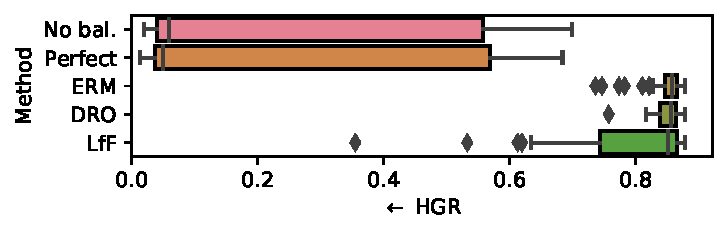
\includegraphics[width=\columnwidth]{figures/cmnist_3dig_4miss_hgr.pdf}\\
  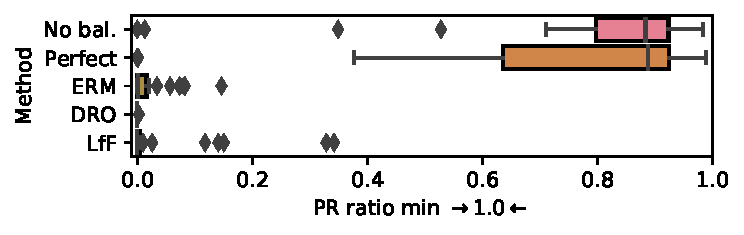
\includegraphics[width=\columnwidth]{figures/cmnist_3dig_4miss_prr-min.pdf}
  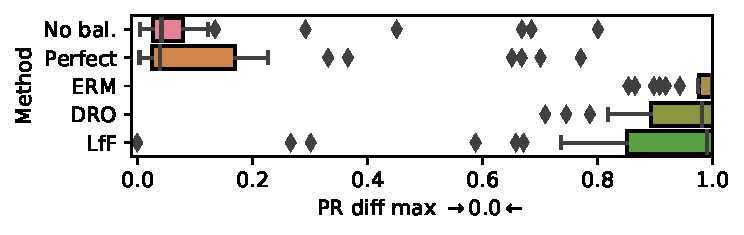
\includegraphics[width=\columnwidth]{figures/cmnist_3dig_4miss_prd-max.pdf}
  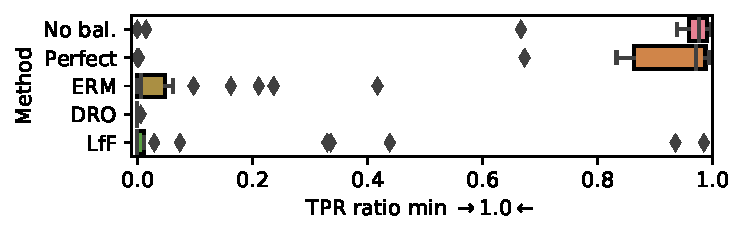
\includegraphics[width=\columnwidth]{figures/cmnist_3dig_4miss_tprr-min.pdf}
  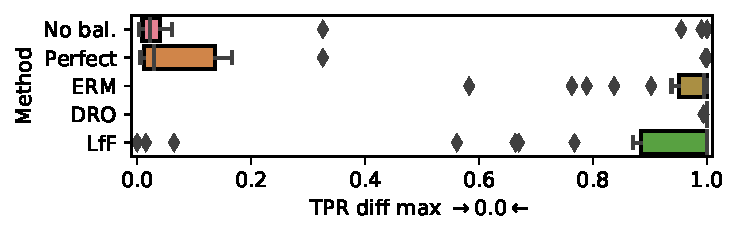
\includegraphics[width=\columnwidth]{figures/cmnist_3dig_4miss_tprd-max.pdf}
  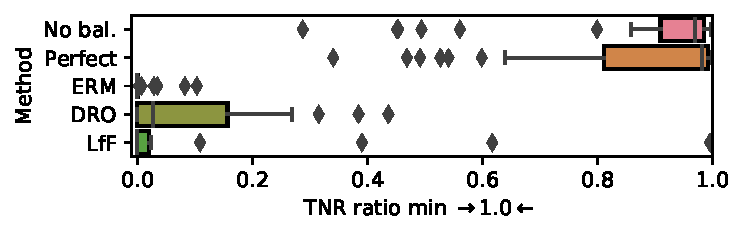
\includegraphics[width=\columnwidth]{figures/cmnist_3dig_4miss_tnrr-min.pdf}
  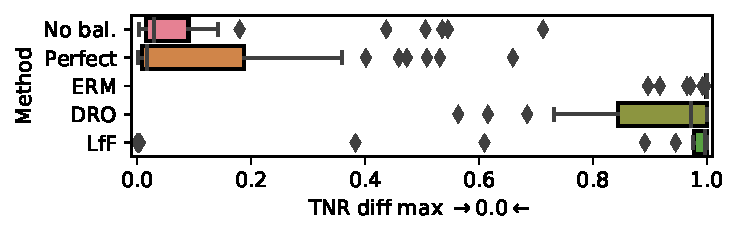
\includegraphics[width=\columnwidth]{figures/cmnist_3dig_4miss_tnrd-max.pdf}
  \caption{
    Results from \textbf{30 repeats} for the Coloured MNIST dataset with three digits: `2', `4' and `6'.
    Four combinations of digit and colour are missing: {\color{green}green} 2's, {\color{blue}blue} 2's, {\color{blue}blue} 4's and {\color{green}green} 6's.
    % \textbf{First row}: Hirschfeld-Gebelein-R\'enyi maximal correlation between $S$ and $Y$.
    \textbf{First row, left}: minimum of all positive rate ratios.
    \textbf{First row, right}: maximum of all positive rate differences.
    \textbf{Second row, left}: minimum of all true positive rate ratios.
    \textbf{Second row, right}: maximum of all true positive rate differences.
    \textbf{Third row, left}: minimum of all true negative rate ratios.
    \textbf{Third row, right}: maximum of all true negative rate differences.
  }%
  \label{fig:cmnist-3dig-4miss-add}
\end{figure*}
\begin{figure*}[htp]
  \centering
%   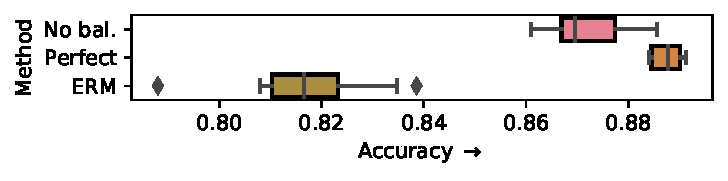
\includegraphics[width=\columnwidth]{figures/celeba_gender_smiling_acc.pdf}
%   \includegraphics[width=\columnwidth]{figures/celeba_gender_smiling_pr.pdf}
  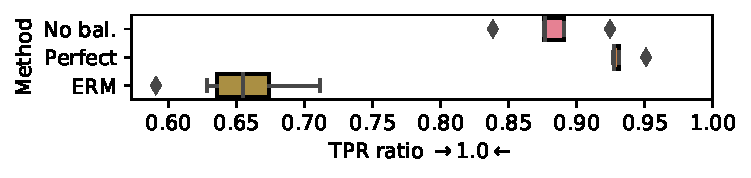
\includegraphics[width=\columnwidth]{figures/celeba_gender_smiling_tprr.pdf}
  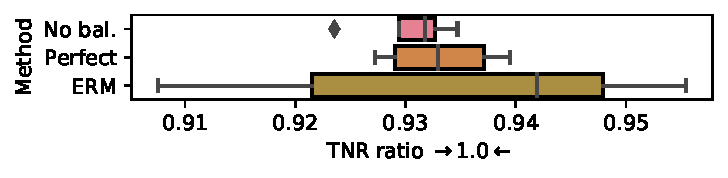
\includegraphics[width=\columnwidth]{figures/celeba_gender_smiling_tnrr.pdf}
  \caption{
    Results from \textbf{10 repeats} for the CelebA dataset with the \emph{subgroup bias} setting.
    The task is to predict ``smiling'' vs ``non-smiling'' and the subgroups are based on gender.
    The subgroup ``female'' is missing samples for the ``smiling'' class.
    % \textbf{Top left}: Accuracy.
    % \textbf{Top right}: Positive rate ratio.
    \textbf{Left}: True positive rate ratio.
    \textbf{Right}: True negative rate ratio.
  }%
  \label{fig:celeba-gender-smiling-add}
\end{figure*}

\subsection{Clustering with an incorrect number of clusters}\label{sec:overclustering}
We also investigate what happens when the number of clusters is set incorrectly.
For 2-digit Coloured MNIST, we expect 4 clusters, corresponding to the 4 possible combinations of the binary class label $y$ and the binary subgroup label $s$.
However, there might be circumstances where the correct number of clusters is not known; how does the batch balancing work in this case?
We run experiments with the number of clusters set to 6 and to 8, while otherwise not changing any part of the method.
It should be noted that this is a very na\"ive way of dealing with an unknown number of clusters.
There are methods specifically designed for identifying the right number of clusters \citep{hamerly2004learning,chazal2013persistence},
and that is what would be used if this situation came up in practice.

The results can be found in figures~\ref{fig:cmnist-2v4-partial-add} and \ref{fig:cmnist-2v4-miss-s-add}.
Bags and batches are constructed by drawing an equal number of samples from each cluster.
Unsurprisingly, the method performs worse than with the correct number of clusters.
When investigating how the clustering methods deal with the larger number of clusters,
we found that it is predominantly those samples that do not appear in the training set
which get spread out among the additional clusters.
This is most likely due to the fact that the clustering is semi-supervised,
with those clusters that occur in the training set having supervision.
The overall effect is that the samples which are not appearing in the training set are overrepresented in the drawn bags,
which means it is easier for the adversary to identify where the bags came from,
and the encoder cannot properly learn to produce an invariant encoding.

% \begin{table*}[tp]
%   \centering
%   \caption{
%     Results on Colored MNIST dataset for a 3-digits-3-colors task, i.e. classification of the digits \emph{two} versus \emph{four} vs \emph{six} with a protected attribute that can take three values ({\color{purple}purple}, {\color{green}green}, {\color{blue}blue}).
%     We consider the scenarios of learning with subgroup bias with four sources missing (30 repeats). 
%   }
%   \label{tab:colormnist3_sup}
%   \scalebox{0.79}{
%   \begin{tabular}{lccccccc}
%     \hline
%     \multicolumn{6}{c}{}\\
%     \multicolumn{6}{c}{Learning with subgroup bias, the sources
%     $\mathcal{M}_{y=\text{'two'},s=\color{green}green}$,
%     $\mathcal{M}_{y=\text{'two'},s=\color{blue}blue}$,
%     $\mathcal{M}_{y=\text{'four'},s=\color{blue}blue}$ and
%     $\mathcal{M}_{y=\text{'six'},s=\color{green}green}$
%     are invisible.}\\
%     \multicolumn{6}{c}{}\\
%     \hline
%     %
%                                          &         AR min. ratio& TPR min. ratio & TNR min. ratio &   AR max. diff &  TPR max. diff &   TNR max. diff \\
%                              \texttt{ZSF} &    0.604 $\pm$ 0.213 &  0.866 $\pm$ 0.176 &  0.702 $\pm$ 0.292 &  0.236 $\pm$ 0.189 &  0.133 $\pm$ 0.175 &  0.297 $\pm$ 0.291 \\
%  \texttt{DRO \cite{HasSriNamLia18}} &     0.027 $\pm$ 0.05 &  0.077 $\pm$ 0.145 &  0.128 $\pm$ 0.147 &  0.887 $\pm$ 0.101 &  0.923 $\pm$ 0.145 &  0.871 $\pm$ 0.147 \\
%   \texttt{Kamiran \& Calders (2012) CNN} &    0.072 $\pm$ 0.077 &  0.208 $\pm$ 0.217 &  0.039 $\pm$ 0.054 &  0.904 $\pm$ 0.087 &  0.792 $\pm$ 0.217 &  0.961 $\pm$ 0.054 \\
%     \hline
%     \hline
%   \end{tabular}}
% \vspace{-0.5cm}
% \end{table*}
% \bibliography{bibfile}
% \bibliographystyle{icml2021}
% \end{document}
